\documentclass[thesis.tex]{subfiles}

\begin{document}

% ----------------------------------------------------------
\chapter{Experiments and results} \label{chap:experiments}
% ----------------------------------------------------------
% Present your results and findings
% ----------------------------------------------------------
In this section, we will first describe our experiment details. We will then present our ..?
Lastly, we demonstrate the surprising improvements of our models on domain specific image classification tasks with Hyper-Kvasir and Hyper-CapsuleCam datasets.




\section{Keeping track of experiments}
% write about logging etc
% ----------------------------------------------------------
Training multiple networks using a wide range of hyperparameters can become chaotic. To overcome this issue we have all our hyperparameters stored in a single python dictionary which easily can be stored in a configuration file. This dictionary handles all hyperparameters, as well as differentiate teacher models from student models, the number of samples and how the number changes during the iterative process of a teacher-student model. One of the parameters in this configuration dictionary is where the log directory is placed. For every run we dedicate a directory for saving all plots, lists, evaluation metrics and trained models and its weights so that we can keep track of what experiments have been run in the past, and what the results where. This log directory became very handy in the case of 'out of memory' errors, in which we could go back and load a trained model, or pseudo labels generated from running through the unlabeled dataset, saving us from having to run experiments multiple times.



\section{Evaluation method and metrics}
% write how we evaluated our model
% ----------------------------------------------------------



% ----------------------------------------------------------
\section{Training details}
% use this section to write about how we managed to get a good classifier
% batch_size, epoch_number, optimizer, dropout, model, image size and other hyper parameters
% ----------------------------------------------------------
% Introduction

% Batch size
For labeled images we re-scale the images to 128 by 128 pixel to reduce memory usage during training. For the smallest model, EfficientNetB0 with 4.7 million parameters, we use a batch size of 128 by default and reduce the batch size when we could not fit the model into the memory. The largest model, EfficientNetB7 with 65.4 million parameters, we reduce the batch size to 32. We find that using a batch size of 256, 128, 64 and 32 leads to the same performance as long as the dataset are resampled. When the data have dominant class imbalances the smaller batch sizes would lead to faster overfitting than the large ones.

% Epochs and training steps
We determine the number of training steps and the learning rate schedule by the batch size for labeled images. The training steps used are calculated by $$ steps = \frac{ds\_size}{bs} $$ where $ds\_size$ is the number of samples in the given train/test/val dataset and $bs$ is the value for batch size we are using. We find that the network have tendencies to overfit the training data when we use a large value for epochs (see Figure \ref{fig:overfit} for an example). Because of this we use early stopping from the tf.keras.callbacks.EarlyStopping package. This  monitors the validation loss during training, and if the model don't improve for 5 epochs the training is terminated and the epoch with the lowest loss, and therefor the best weights, is restored. Depending om model size we use, this would happen somewhere around epoch number 30. The larger model would take longer to hit early stopping threshold than the smaller ones.

% notice; used high learning rate (0.01), low dropout and aug_mult
\begin{figure} % fig:overfit
  \begin{center}
    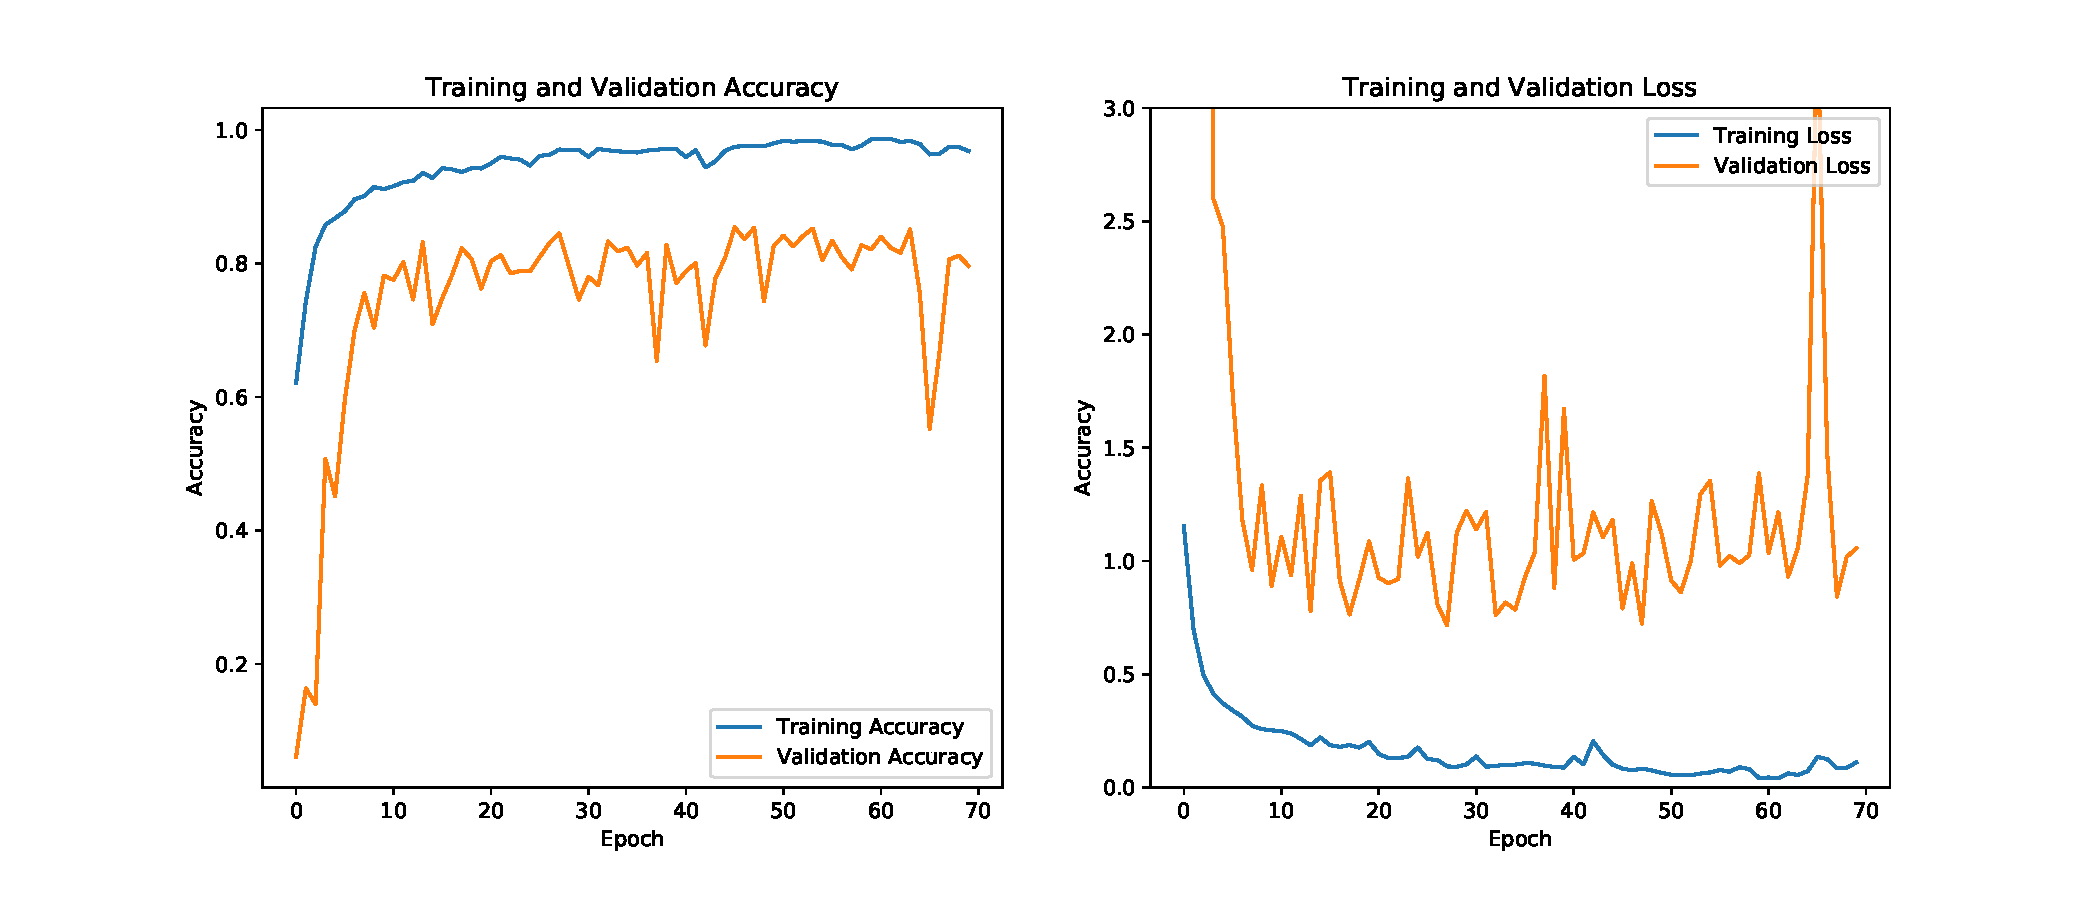
\includegraphics[width=.7\textwidth]{overfit}
    \caption[Example where the model accuracy for training data greatly outperforms the accuracy for testing data]{Example where the model accuracy for training data greatly outperforms the accuracy for testing data.}
    \label{fig:overfit}
  \end{center}
\end{figure}

% Optimizer and learning rate
The optimizer we use is for our experiments are Adam \cite{AdamMethod17}, we use this optimizer because it has shown to perform well for image classification tasks in other studies. Compared to SGD algorithm we get a stable accuracy gain for every epoch and the loss converges quickly. By default in Keras the learning rate for Adam is set to 0.001, this is a good starting point for us as well. Although Adam uses an adaptive learning rate we manage to get slightly better results by starting the learning rate at 0.01, and then using inverse time decay (another Learning Rate Scheduler), with a steep learning rate drop-off in the first epochs and then the learning rate plateau after about 10 epochs.

% Base model, dropout etc
For our experiments we are more concerned with the possibility of improving medical image classification tasks with greatly imbalanced datasets than getting state-of-the-art results. We therefore use the tested and proven EfficientNet for our training. This model suits us good for two reasons (1), it comes with pretrained ImageNet weights, and (2) it is easy to test different model sizes. The EfficientNets (B0-B7) are used for all our experiments. This base model is then connected with a pooling layer, a dropout layer, a fully connected layer, another dropout layer and finally a output layer. The dropout is set to 10\% for the case of training the teacher model, and 30\% for the training the student model on the combined labeled data and generated pseudo labels. 

% Dropout and augmentation
We find that by using dropout and image augmentation the model generalizes much better to the validation data, and the teacher model is better at learning the features for the minority classes, which are only represented by a few samples in the training data. For training the teacher model we use image augmentation multiplier set to 10\% and after switching the teacher with the student we increase the image augmentation multiplier to 100\%.



\subsection{Labeled and labeled dataset}
% Specify which datasets we used to run our experiments
% ----------------------------------------------------------
We conduct experiments on Hyper-Kvasir dataset since it is open-source and to the best of our knowledge, the largest colonoscopy dataset available. We filter the images into three datasets for training, testing and validation purposes. The data is split so that 60\% of the images go to training, 15\% go to test data and the remaining 15\% go to validation. The training dataset is reduced to 128 by 128 pixels with bilinear interpolation, shuffled, batched and augmented.

The unlabeled dataset contain 100 thousand images, and the corpus of images are taken from a wide variety of colonoscopies.This dataset is used for generating new pseudo labels which will later be concatenated with the training data. Due to memory and time restrictions we only keep the images which get a probability score for one of the domain classes of 90\% and above, the images which receive a lower probability score are considered out of domain images. we then sort the unlabeled data by the probability score within each of Hyper-Kvasir's 23 classes.



\subsection{Architecture}
% Base model, EfficientNets
% ----------------------------------------------------------
We use EfficientNets at the base of our model since it handles large datasets exceptionally well. 




% ----------------------------------------------------------
\section{Experiments}
%
% ----------------------------------------------------------


\section{Binary vs multiclass}
% Perhaps skip if it requires to much effort and time to make data binary..
% ----------------------------------------------------------



\subsection{Weight initialization}
% initializing the model with weights vs without weigts.
% initializing the student with the teacher model's weights?
% mention imagenet weights are trained using autoAugment
% ----------------------------------------------------------
Found that training on Hyper-Kvasir datasets yield best results when using EfficientNet with is initialized with weights from ImageNet. Early in our study the only pre-trained weights readily available were trained without the use of AutoAugment, and performed slightly worse than the ImageNet weights trained with AutoAugment, released at a later time. Especially we observed that the model would initialize the training with lower loss when trained with ImageNet-AutoAugment weigths.

%TODO insert plot of training loss and accuracy (and class-report?) of imagenet-autoaugment and imagenet

We tested with initializing the teacher model with original noisy-student weights but found that loss were fluxing more early in training. Also when trained for same number of epochs as with ImageNet weights the model would perform worse on the evaluation data, with lower accuracy and lower recall.

%TODO insert plot of training loss and accuracy (and class-report?) of noisy-student

As part of this experiment we also tested with initializing the teacher model with no weights and train from scratch. Not surprisingly, this gave slower training, and after 20 epochs we got a 15\% lower accuracy than when training with ImageNet weights.



\subsection{Class Weigting vs Resample}
Found that by re-sampling the dataset the model generelized much better than by calculating the loss from weighted class distribution.




\subsection{Model complexity}
% how model size effects how the teacher model learns






% ----------------------------------------------------------
\section{Teacher-student model}
% section for everything teacher-student
% ----------------------------------------------------------



\subsection{Noising the student}



\subsection{Model size}
% Test how model size effects the performance of teacher/student model
% a; small model vs large model
% b; iterative larger model during training
% ----------------------------------------------------------





\subsection{Number of iterations}
% how many iterations of swapping student with teacher to get good results?
% ----------------------------------------------------------





% ----------------------------------------------------------
\section{Results} \label{sec:C4-results}
% ----------------------------------------------------------






% ----------------------------------------------------------
\section{Summary} \label{sec:C4-summary}
% ----------------------------------------------------------




\end{document}